\chapter{Explorar nuestro entorno}\label{ch:g6:exploring-our-environment}

Cruza el patio del colegio un mediodía de julio y la cara sur del muro
estará caliente bajo tu mano, el aire sobre el asfalto tembloroso, y
lo único verde a la vista será una hierba en una grieta. Pasa detrás
del muro norte: aire fresco, tierra húmeda, musgo, cochinillas bajo
una piedra. Dos mundos a tres metros uno de otro. Este curso empieza
explorando \omterm{def:g6:exploring-our-environment:components}{entornos} como lo hacen los científicos --- midiéndolos y
preguntándose por qué cada \omterm{def:g6:exploring-our-environment:components}{ser vivo} vive exactamente donde vive.

\section{De qué está hecho un entorno}

\begin{definition}[Los componentes de un entorno]\label{def:g6:exploring-our-environment:components}
Un \emph{entorno}\index{entorno} --- un patio, un bosque, la orilla de
una charca --- contiene tres clases de componentes:
\begin{enumerate}
  \item los \emph{seres vivos}\index{ser vivo}: los \omterm{def:g1:animals-around-us:animal}{animales}, las
        \omterm{def:g1:plants-around-us:plant}{plantas}, las setas y la vida microscópica presentes;
  \item la \emph{materia mineral}\index{materia mineral}, que no
        estuvo nunca viva: roca, piedra, la parte mineral de la
        tierra, agua, aire;
  \item las \emph{huellas y los restos} de seres vivos: \omterm{def:g1:plants-around-us:parts}{hojas} muertas,
        madera caída, excrementos, \omterm{def:g1:animals-around-us:covering}{plumas}, \omterm{def:g1:animals-around-us:covering}{conchas} --- la caja del
        ``estuvo vivo'' de la \cref{def:g1:living-or-not:nonliving},
        ahora un juego de pistas para quien explora.
\end{enumerate}
\end{definition}

\begin{example}[Inventario detrás del muro norte]\label{ex:g6:exploring-our-environment:inventory}
Diez minutos de inventario en el rincón fresco: \omterm{def:g6:exploring-our-environment:components}{seres vivos} --- musgo,
\omterm{prop:g4:plants-without-seeds:damp}{helechos}, cochinillas, un caracol, un ciempiés, hiedra; mineral --- la
piedra del muro, tierra húmeda, un charco; huellas --- \omterm{def:g1:plants-around-us:parts}{hojas} muertas,
una \omterm{def:g1:animals-around-us:covering}{concha} de caracol, excrementos de pájaro en la albardilla. Tres
listas, y el rincón queda descrito como el sitio de trabajo de una
científica.
\end{example}

\begin{omfigure}
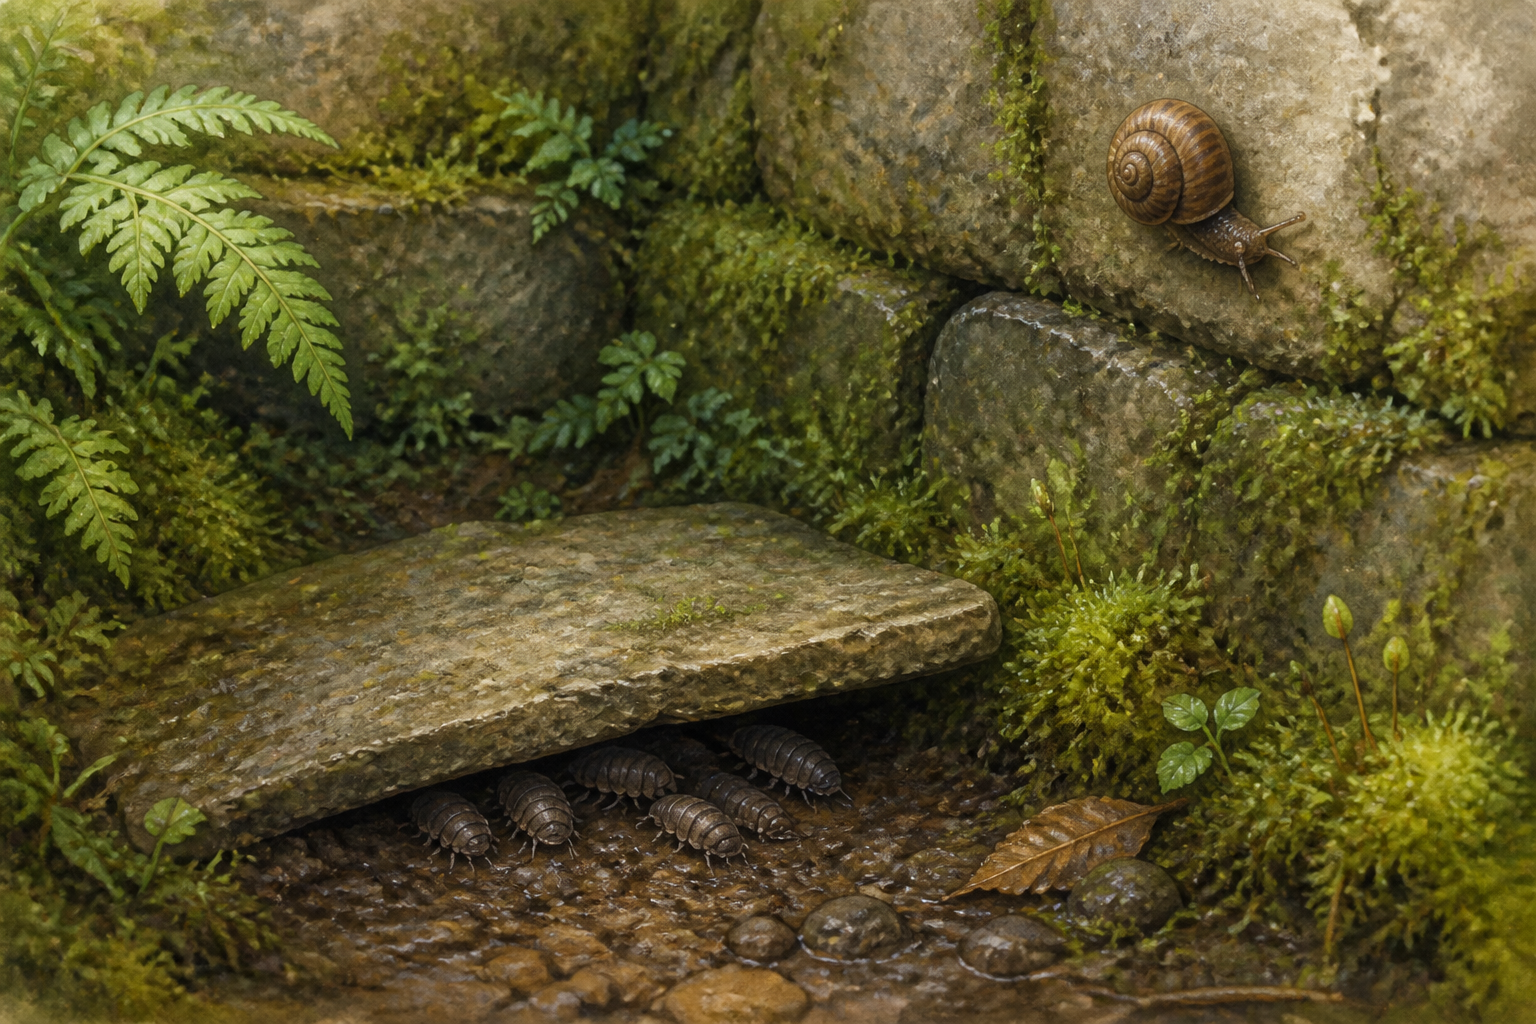
\includegraphics[width=0.62\linewidth]{images/book1/ai/g6-env-wallcorner.png}

{\small El rincón fresco, a medio inventario: musgo, \omterm{prop:g4:plants-without-seeds:damp}{helechos}, un
caracol sobre la piedra --- y bajo la losa levantada, el \omterm{def:g6:exploring-our-environment:microhabitat}{microhábitat}
de las cochinillas (vuelve a ponerla).}
\end{omfigure}

\begin{remark}[Las huellas cuentan como datos]\label{rem:g6:exploring-our-environment:traces}
Casi todos los \omterm{def:g1:animals-around-us:animal}{animales} se esconden o huyen, así que quien explora lee
a menudo \emph{huellas} en su lugar: una avellana roída nombra al
ratón de campo, una telaraña nombra a su dueña, unas pisadas en el
barro nombran a la garza. Un inventario que solo enumera lo que se
estuvo quieto para dejarse ver se pierde a la mitad de los habitantes.
\end{remark}

\section{Medir las condiciones}

\begin{definition}[Condiciones del entorno]\label{def:g6:exploring-our-environment:conditions}
Las \emph{condiciones}\index{condiciones (del entorno)} de un \omterm{def:g6:exploring-our-environment:components}{entorno}
son sus características físicas medibles:
\begin{itemize}
  \item la \emph{temperatura}\index{temperatura}, medida con un
        termómetro, en grados Celsius;
  \item la \emph{humedad}\index{humedad} --- lo húmedos que están el
        aire o la tierra;
  \item la \emph{luz}\index{luz (condición)} --- desde el pleno sol
        hasta la sombra profunda.
\end{itemize}
Las condiciones cambian de un punto a otro --- a menudo bruscamente en
unos metros --- y a lo largo del día y del año.
\end{definition}

\begin{example}[El patio, medido]\label{ex:g6:exploring-our-environment:measured}
El reconocimiento de aquel mediodía de julio, con instrumentos: al pie
del muro sur --- \qty{38}{\degreeCelsius}, seco, pleno sol; en el
rincón norte --- \qty{22}{\degreeCelsius}, tierra húmeda, sombra
profunda. Tres metros de distancia, dieciséis grados de diferencia.
Los dos mundos del primer párrafo son ya dos \emph{filas de una tabla}
--- y eso es un avance, porque las tablas se pueden comparar.
\end{example}

\begin{proposition}[Las condiciones deciden a los habitantes]\label{prop:g6:exploring-our-environment:decide}
Los \omterm{def:g6:exploring-our-environment:components}{seres vivos} de un punto se ajustan a sus \omterm{def:g6:exploring-our-environment:conditions}{condiciones}: cada \omterm{def:g5:biodiversity:species}{especie}
prospera solo dentro de su propio intervalo de \omterm{def:g6:exploring-our-environment:conditions}{temperatura}, \omterm{def:g6:exploring-our-environment:conditions}{humedad} y
\omterm{def:g6:exploring-our-environment:conditions}{luz}. El musgo y las cochinillas necesitan \omterm{def:g6:exploring-our-environment:conditions}{humedad} (la cubierta de la
cochinilla, a diferencia de la de un insecto, deja escapar el agua ---
se seca mortalmente en una hora de sol); la hierba de la grieta
aguanta la sequía y el resplandor. Donde las \omterm{def:g6:exploring-our-environment:conditions}{condiciones} son
distintas, los habitantes son distintos --- la regla que hay detrás de
todos los \omterm{def:g2:where-animals-live:habitat}{hábitats} del \cref{ch:g2:where-animals-live}.
\end{proposition}
\admitted

\begin{example}[La caja que eligen las cochinillas]\label{ex:g6:exploring-our-environment:chooser}
El experimento clásico: una caja cerrada, con una mitad forrada de
papel húmedo y la otra de papel seco, y una docena de cochinillas
soltadas a lo largo del centro. En unos minutos, casi todas están en
el lado húmedo. Repítelo con una mitad en sombra frente a una mitad
iluminada: se juntan en la sombra. Nadie las lleva en rebaño --- cada
\omterm{def:g1:animals-around-us:animal}{animal}, dando vueltas y girando, acaba donde su cuerpo está a gusto.
El mapa de las cochinillas \emph{es} un mapa de la \omterm{def:g6:exploring-our-environment:conditions}{humedad}.
\end{example}

\begin{method}[Reconocer un sitio]\label{met:g6:exploring-our-environment:survey}
Para reconocer un sitio pequeño como una científica de campo:
\begin{enumerate}
  \item elige y marca una zona pequeña --- un metro cuadrado bien
        rebuscado dice más que una hectárea vista de pasada;
  \item mide las \omterm{def:g6:exploring-our-environment:conditions}{condiciones}: \omterm{def:g6:exploring-our-environment:conditions}{temperatura}, \omterm{def:g6:exploring-our-environment:conditions}{humedad}, \omterm{def:g6:exploring-our-environment:conditions}{luz} --- con los
        mismos instrumentos y de la misma manera en cada sitio (la
        regla de justicia del \cref{met:g4:what-plants-need:fairtest});
  \item inventaría las tres clases de componentes --- \omterm{def:g6:exploring-our-environment:components}{seres vivos},
        \omterm{def:g6:exploring-our-environment:components}{materia mineral}, huellas --- rebuscando como es debido: bajo
        las piedras (vuelve a ponerlas:
        \cref{met:g2:caring-for-nature:rules}), en las grietas, en el
        envés de las \omterm{def:g1:plants-around-us:parts}{hojas};
  \item anótalo todo allí mismo --- listas, dibujos, recuentos; la
        memoria no es un instrumento de registro;
  \item compara los sitios: empareja cada diferencia de habitantes con
        una diferencia de \omterm{def:g6:exploring-our-environment:conditions}{condiciones}.
\end{enumerate}
\end{method}

\begin{remark}[Por qué las anotaciones ganan a los recuerdos]\label{rem:g6:exploring-our-environment:records}
De vuelta bajo techo, dos personas que se fiaron de la memoria
discutirán sobre si los caracoles eran tres o cinco. El cuaderno lo
zanja --- o reconoce con honradez que no se contaron los caracoles.
Las anotaciones escritas, hechas en el sitio, son lo que convierte un
paseo en datos; todas las ciencias de este libro funcionan con ellas.
\end{remark}

\section{Un entorno, muchos micromundos}

\begin{definition}[Microhábitat]\label{def:g6:exploring-our-environment:microhabitat}
Dentro de un mismo \omterm{def:g6:exploring-our-environment:components}{entorno}, cada punto pequeño con sus propias
\omterm{def:g6:exploring-our-environment:conditions}{condiciones} y sus propios habitantes --- el envés de una piedra, una
grieta del muro, el pie sombrío del seto --- es un
\emph{microhábitat}\index{microhábitat}. Los pisos del bosque de la
\cref{rem:g2:where-animals-live:layers} eran microhábitats; el metro
cuadrado de quien reconoce el terreno suele tener varios.
\end{definition}

\begin{example}[La piedra, por arriba y por abajo]\label{ex:g6:exploring-our-environment:stone}
Una piedra del rincón fresco: encima, líquenes y una mosca tomando el
sol --- iluminado, seco, cálido. Debajo, cochinillas, un ciempiés,
raicillas pálidas --- oscuro, húmedo, fresco. Dos \omterm{def:g6:exploring-our-environment:microhabitat}{microhábitats}
completos separados por cinco centímetros de roca, cada uno habitado
justamente por aquellos \omterm{def:g6:exploring-our-environment:components}{seres vivos} cuyos intervalos encajan con sus
\omterm{def:g6:exploring-our-environment:conditions}{condiciones}.
\end{example}

\section{Ejercicios}

\begin{exercise}[$\star$]\label{exo:g6:exploring-our-environment:1}
Nombra las tres clases de componentes de un \omterm{def:g6:exploring-our-environment:components}{entorno}, con dos ejemplos
de cada una sacados del inventario del rincón norte.
\end{exercise}

\begin{exercise}[$\star$]\label{exo:g6:exploring-our-environment:2}
¿Qué \omterm{def:g6:exploring-our-environment:conditions}{condiciones} mide una científica de campo en un sitio y con qué
(donde se haya nombrado un instrumento)?
\end{exercise}

\begin{exercise}[$\star$]\label{exo:g6:exploring-our-environment:3}
Clasifica en las tres clases de componentes: un helecho, una \omterm{def:g1:animals-around-us:covering}{concha} de
caracol, un charco, excrementos de pájaro, un ciempiés, la piedra del muro.
\end{exercise}

\begin{exercise}[$\star$]\label{exo:g6:exploring-our-environment:4}
A partir del \cref{ex:g6:exploring-our-environment:measured}: ¿cuáles
son las diferencias de \omterm{def:g6:exploring-our-environment:conditions}{temperatura} y de \omterm{def:g6:exploring-our-environment:conditions}{luz} entre los dos puntos? ¿Qué
habitantes encajan con cada uno?
\end{exercise}

\begin{exercise}[$\star$]\label{exo:g6:exploring-our-environment:5}
¿Por qué se muere una cochinilla en una hora de sol y qué explica eso
sobre dónde se encuentran las cochinillas?
\end{exercise}

\begin{exercise}[$\star$]\label{exo:g6:exploring-our-environment:6}
Nombra tres huellas y el \omterm{def:g1:animals-around-us:animal}{animal} que nombra cada una, como en la
\cref{rem:g6:exploring-our-environment:traces}.
\end{exercise}

\begin{exercise}[$\star\star$]\label{exo:g6:exploring-our-environment:7}
Describe el experimento de la caja que eligen las cochinillas: montaje,
resultado y qué demuestra --- sin que nadie las lleve en rebaño.
\end{exercise}

\begin{exercise}[$\star\star$]\label{exo:g6:exploring-our-environment:8}
¿Por qué hay que medir las \omterm{def:g6:exploring-our-environment:conditions}{condiciones} de la misma manera en cada
sitio? ¿De qué método anterior es esta la versión de campo?
\end{exercise}

\begin{exercise}[$\star\star$]\label{exo:g6:exploring-our-environment:9}
Da los dos \omterm{def:g6:exploring-our-environment:microhabitat}{microhábitats} de la piedra del
\cref{ex:g6:exploring-our-environment:stone}, con sus \omterm{def:g6:exploring-our-environment:conditions}{condiciones} y un
habitante de cada uno.
\end{exercise}

\begin{exercise}[$\star\star$]\label{exo:g6:exploring-our-environment:10}
Un reconocimiento anota ``algunos bichos, hacía calorcillo''. Reescribe
las instrucciones con el \cref{met:g6:exploring-our-environment:survey}
--- ¿qué se debería haber hecho en cada paso?
\end{exercise}

\begin{exercise}[$\star\star$]\label{exo:g6:exploring-our-environment:11}
La hiedra sube por el muro norte pero no por el sur. Propón una
explicación con la forma de la
\cref{prop:g6:exploring-our-environment:decide}, y una observación o
una medida que la pondrían a prueba.
\end{exercise}

\begin{exercise}[$\star\star\star$]\label{exo:g6:exploring-our-environment:12}
En la caja de las cochinillas, un alumno objeta: ``a lo mejor solo se
juntaron cerca de la pared, y el lado húmedo tenía más pared''. Diseña
una versión mejorada del experimento que responda a la objeción.
(Piensa en la prueba justa.)
\end{exercise}

\section{Problema: Las dos cunetas}

\begin{problem}[{Problema de fin de semana --- el club de
naturalistas reconoce dos cunetas de una carretera y encuentra dos
mundos distintos}]\label{pb:g6:exploring-our-environment:1}
El club de naturalistas reconoce dos cunetas del mismo camino,
separadas $50$ metros. La cuneta N va por el lado norte de un seto
alto; la cuneta S va a campo abierto, mirando al sur. El club trabaja
como manda el manual: mismos instrumentos, mismo metro cuadrado por
sitio, mismo tiempo de búsqueda.

\medskip\noindent\textbf{Parte I --- Las medidas.}
\begin{enumerate}
  \item Los termómetros marcan \qty{19}{\degreeCelsius} en la cuneta N
        y \qty{31}{\degreeCelsius} en la cuneta S a la misma hora.
        ¿Qué único elemento de los sitios explica mejor la diferencia?
  \item La tierra de la cuneta N se pega a los dedos; la de la cuneta
        S se desmenuza en polvo. Traduce las dos observaciones al
        vocabulario de la
        \cref{def:g6:exploring-our-environment:conditions}.
  \item El club mide al mediodía. Da una razón por la que la
        comparación sería menos justa si la cuneta N se midiera al
        mediodía y la cuneta S a las 6 de la tarde.
  \item ¿Por qué usa el club el \emph{mismo} marco de un metro
        cuadrado y el mismo tiempo de búsqueda en los dos sitios?
\end{enumerate}

\medskip\noindent\textbf{Parte II --- Los inventarios.}
\begin{enumerate}[resume]
  \item Lista de la cuneta N: musgo, \omterm{prop:g4:plants-without-seeds:damp}{helechos}, cochinillas, caracoles,
        un sapo. Lista de la cuneta S: hierbas secas, una hierba grande
        de \omterm{def:g1:plants-around-us:parts}{hojas} cerosas, hormigas, una lagartija tomando el sol,
        saltamontes. Clasifica los miembros de cada lista en las tres
        clases de componentes --- y fíjate en lo que les falta a las
        listas (repasa la
        \cref{def:g6:exploring-our-environment:components}).
  \item Para las cochinillas, el sapo y la lagartija, di con qué
        cuneta encajan sus necesidades y por qué (usa la
        \cref{prop:g6:exploring-our-environment:decide} y lo que sabes
        de cada \omterm{def:g1:animals-around-us:animal}{animal}).
  \item En la cuneta S el club encuentra una \omterm{def:g1:animals-around-us:covering}{concha} de caracol, pero
        ningún caracol, y se pregunta si allí viven caracoles. ¿Qué
        dos posibilidades honradas deja abiertas una huella así?
  \item Bajo una piedra plana de la cuneta N: ocho cochinillas, un
        ciempiés, raicillas blancas. Nombra las \omterm{def:g6:exploring-our-environment:conditions}{condiciones} del
        \omterm{def:g6:exploring-our-environment:microhabitat}{microhábitat} y enuncia la regla que puso allí a esos habitantes.
\end{enumerate}

\medskip\noindent\textbf{Parte III --- La explicación.}
\begin{enumerate}[resume]
  \item Empareja cada diferencia de habitantes con una diferencia de
        \omterm{def:g6:exploring-our-environment:conditions}{condiciones}: completa ``N tiene musgo y sapos porque \dots; S
        tiene lagartijas y hierbas de \omterm{def:g1:plants-around-us:parts}{hojas} cerosas porque \dots''.
  \item Está previsto arrancar el seto. Predice las \omterm{def:g6:exploring-our-environment:conditions}{condiciones} de la
        cuneta N dos veranos después --- y sus habitantes, usando el
        emparejamiento de la pregunta 9.
  \item Un socio propone comprobar la predicción como es debido:
        reconocer las dos cunetas otra vez cuando el seto ya no esté.
        ¿Por qué hay que usar los \emph{mismos} sitios, instrumentos y
        estación para que el nuevo reconocimiento valga?
  \item El informe del club acaba: ``los habitantes cartografían las
        \omterm{def:g6:exploring-our-environment:conditions}{condiciones}''. Explica la frase con la caja que eligen las
        cochinillas (\cref{ex:g6:exploring-our-environment:chooser}) y
        di por qué no hace falta ningún rebaño para que un mapa así se
        dibuje solo.
\end{enumerate}
\end{problem}
